\documentclass[10pt]{article}

\usepackage[letterpaper,margin=0.82in]{geometry}
\usepackage[T1]{fontenc}
\usepackage{lmodern}
\usepackage{inconsolata}
\usepackage{microtype}
\usepackage{graphicx}
\usepackage{subcaption}
\usepackage{float}
\usepackage{booktabs}
\usepackage{tabularx}
\usepackage{array}
\usepackage{enumitem}
\usepackage[table,dvipsnames]{xcolor}
\usepackage[hidelinks]{hyperref}

\definecolor{ink}{HTML}{16324F}
\definecolor{tealaccent}{HTML}{0F766E}
\definecolor{warmbg}{HTML}{F5EFE7}
\definecolor{coolbg}{HTML}{EEF5F6}
\definecolor{lightline}{HTML}{D9E4E7}

\setlength{\parindent}{0pt}
\setlength{\parskip}{0.4em}
\setlist[itemize]{leftmargin=1.25em,itemsep=0.22em,topsep=0.22em}
\setlist[enumerate]{leftmargin=1.25em,itemsep=0.22em,topsep=0.22em}
\pagestyle{plain}

\newcommand{\softpanel}[2]{%
    \fcolorbox{#1!55}{#1!7}{%
        \parbox{\dimexpr\linewidth-2\fboxsep-2\fboxrule\relax}{#2}%
    }%
}

\begin{document}

\begin{center}
    {\Large\bfseries CreditSense: Methods Tried and Project Timeline \par}
    \vspace{0.35em}
    {\normalsize A readable record of the branches, ideas, detours, and score jumps that shaped the final project \par}
    \vspace{0.75em}
    {\small Johnny Izhak Kyriakos \quad | \quad March 2026 working history \par}
\end{center}

\vspace{0.5em}

\noindent
\begin{minipage}[t]{0.60\linewidth}
\softpanel{tealaccent}{%
\textbf{What this report is.} The main report only explains the clean final public solution. This document does the opposite: it keeps the messy history intact enough to understand what was tried, what moved the score, what only looked promising for a moment, and why some branches were kept while others were left behind.

\medskip
\textbf{How the timeline was rebuilt.} The reconstruction comes from saved score tables, result JSON files, long training logs, submission artifacts, and dated project chats. Some early intermediate outputs were overwritten later, so whenever an old exact number is missing, the report says so instead of pretending otherwise.}
\end{minipage}\hfill
\begin{minipage}[t]{0.36\linewidth}
\softpanel{ink}{%
\textbf{Reading guide}
\begin{enumerate}
    \item Timeline first: when the main turns happened.
    \item Methods matrix second: what each lane was trying to do.
    \item Compute notes third: what ran on Mac vs HPC and how long it took.
    \item Final verdict last: what survived into the final project story.
\end{enumerate}

\textbf{One-line summary.} The best gains came from stronger feature artifacts and careful blending of strong tabular branches. Pure novelty for its own sake usually lost.}
\end{minipage}

\vspace{0.9em}

\section*{1. Timeline At A Glance}

The project changed direction a few times, but the main arc was fairly consistent: baseline recovery first, then stronger tree ensembles, then a target-stat branch, then neural or meta layers on top of those tabular sources, and finally a professor-inspired parallel lane to test whether broader feature generation could push the upstream score further.

\softpanel{ink}{%
\textbf{If you only want the short version}
\begin{itemize}
    \item The first reliable jump came from turning the baseline into a stronger tree ensemble, not from chasing exotic models too early.
    \item The most important classical step was the target-stats branch.
    \item The best local score came later from a neural or meta blend on top of strong tabular branches, not from abandoning those branches.
    \item The professor lane improved the refreshed target-stats source a little, but the strongest final local blends still came from the already strong hybrid stack.
\end{itemize}}

\begin{figure}[H]
    \centering
    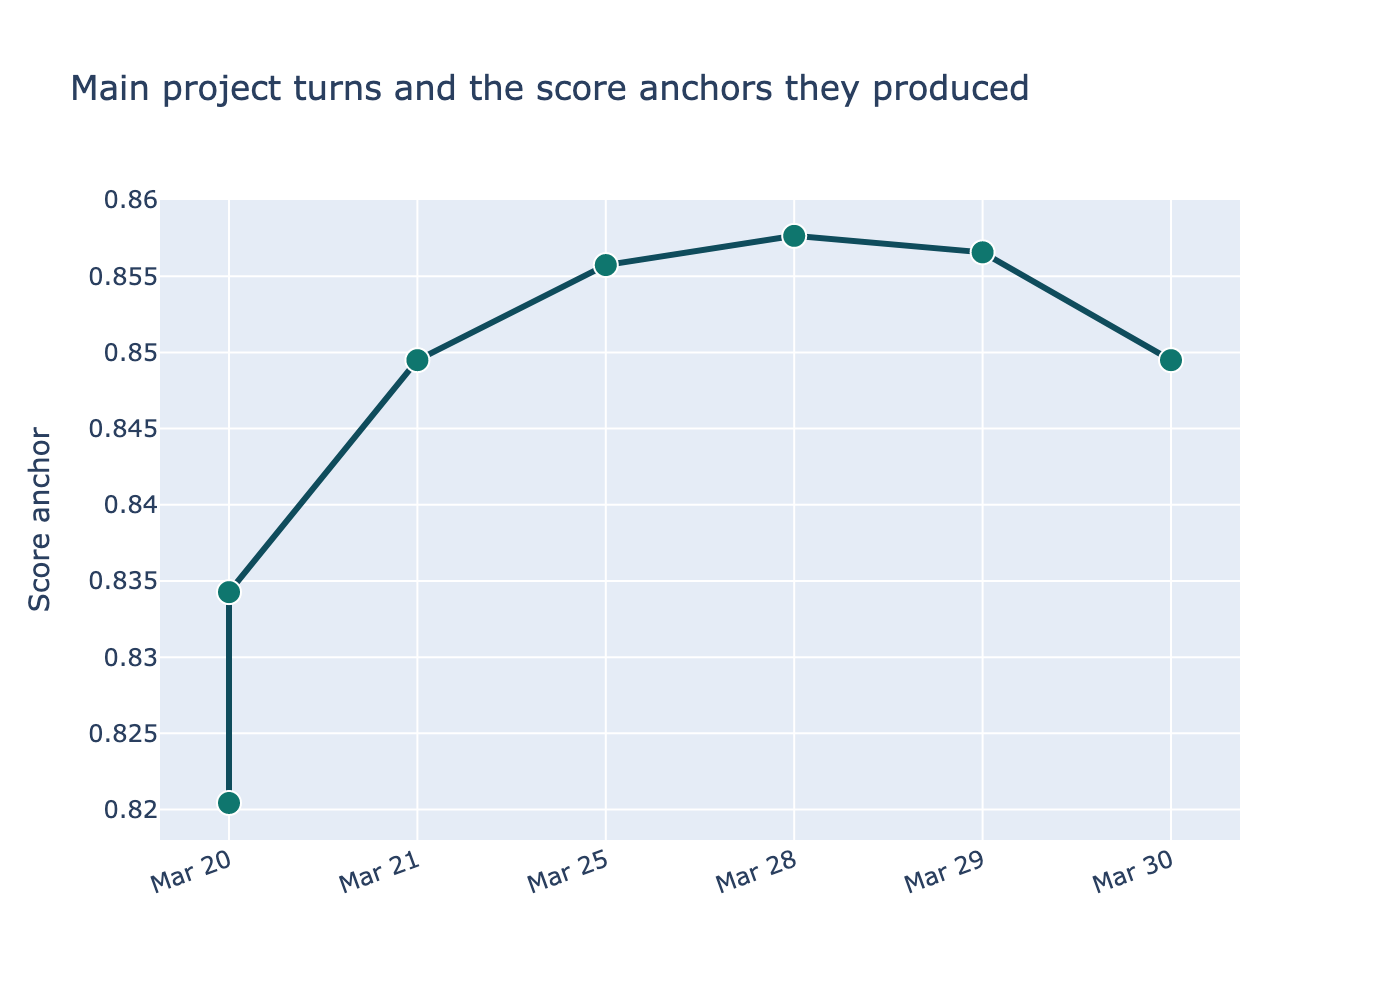
\includegraphics[width=\linewidth]{figures/methods_milestones.png}
    \caption{The main turns in the project, shown with the score anchor each phase produced.}
\end{figure}

\rowcolors{2}{coolbg}{white}
\begin{table}[H]
    \centering
    \small
    \begin{tabularx}{\linewidth}{>{\bfseries}p{0.13\linewidth} >{\raggedright\arraybackslash}p{0.22\linewidth} >{\centering\arraybackslash}p{0.12\linewidth} X}
        \rowcolor{ink!12}
        Date & Phase & Score & What changed \\
        Mar 20 & Baseline reconstruction & 0.82043 public & Recovered the assignment setup, rebuilt the baseline, and used the first Kaggle checks to calibrate the local split. \\
        Mar 20 & Poly-parallel tree blend & 0.834266 & The baseline turned into a broader tree stack, with an extra MPS-supported lane. \\
        Mar 21 & Overnight ensemble & 0.849489 & Tuned XGB, LGB, CatBoost, ExtraTrees, and MPS were combined into the first really systematic ensemble family. \\
        Mar 25 & Target-stats branch & 0.855731 & OOF target statistics and stronger pruning pushed the main classical branch into the mid 0.855 range. \\
        Mar 28 & Neural and meta topping & 0.857645 & The best local score came from a weighted neural/meta blend placed on top of strong tabular branches rather than a fully neural replacement. \\
        Mar 29 & Professor lane & 0.856566 & Broader feature generation and a refreshed target-stats branch improved the upstream source a bit, but did not replace the strongest final blends. \\
        Mar 30 & Public packaging & 0.849489 & The public repo was rebuilt around the cleaner overnight lane because it stayed reproducible and easy to explain. \\
    \end{tabularx}
    \caption{The seven project turns that matter most to the final story.}
\end{table}

Two practical notes shaped the work from early on. First, Kaggle submissions were treated as scarce calibration points rather than as blind search. Second, the repo became dense quickly, so each later stage was judged not only by score, but also by whether it stayed understandable enough to package into a clean final deliverable.

\section*{2. What Each Lane Was Trying To Do}

\rowcolors{2}{white}{warmbg}
\begin{table}[H]
    \centering
    \small
    \begin{tabularx}{\linewidth}{>{\bfseries}p{0.18\linewidth} >{\raggedright\arraybackslash}p{0.24\linewidth} >{\raggedright\arraybackslash}p{0.24\linewidth} X}
        \rowcolor{tealaccent!14}
        Lane & Core idea & Why it was tried & Verdict \\
        Early boosted trees & LightGBM, XGBoost, ExtraTrees, and simple blends on a shared holdout split & Fast way to beat the template and check whether the local validation scheme was trustworthy & It worked well enough to calibrate Kaggle quickly and became the foundation for the next families. \\
        Poly parallel + MPS & Broader engineered features plus an extra MPS-supported branch & Test whether wider but still readable feature work could move the score before deeper refactors & It improved on the baseline and made branch-first thinking natural. \\
        Overnight ensemble & Tuned XGB, LGB, CatBoost, ExtraTrees, MPS, and a learned combiner & Build one serious tabular family instead of many half-related scripts & This became the cleanest strong lane and later the public-facing path. \\
        Target-stats family & OOF target statistics, stronger pruning, and richer tabular blending & Push the classical branch as far as possible before giving up on feature-side work & This became the main upstream source for the strongest local hybrids. \\
        Neural and meta layers & Wide-deep, residual MLP, classifier-only blend, meta stack, and weighted blend & Check whether neural or meta layers could squeeze more value out of strong tabular predictions & Light meta layers helped. Fully replacing the tabular core usually did not. \\
        Professor lane & Broader feature factory, stronger missingness features, classical screening, and GA-style refinement after pruning & Systematically test the professor's suggestions without throwing away the current winners & Useful as an upstream refinement lane, but not a clean replacement for the strongest final blends. \\
    \end{tabularx}
    \caption{The main branches were not random. Each lane was trying to answer a fairly specific question.}
\end{table}

\begin{figure}[H]
    \centering
    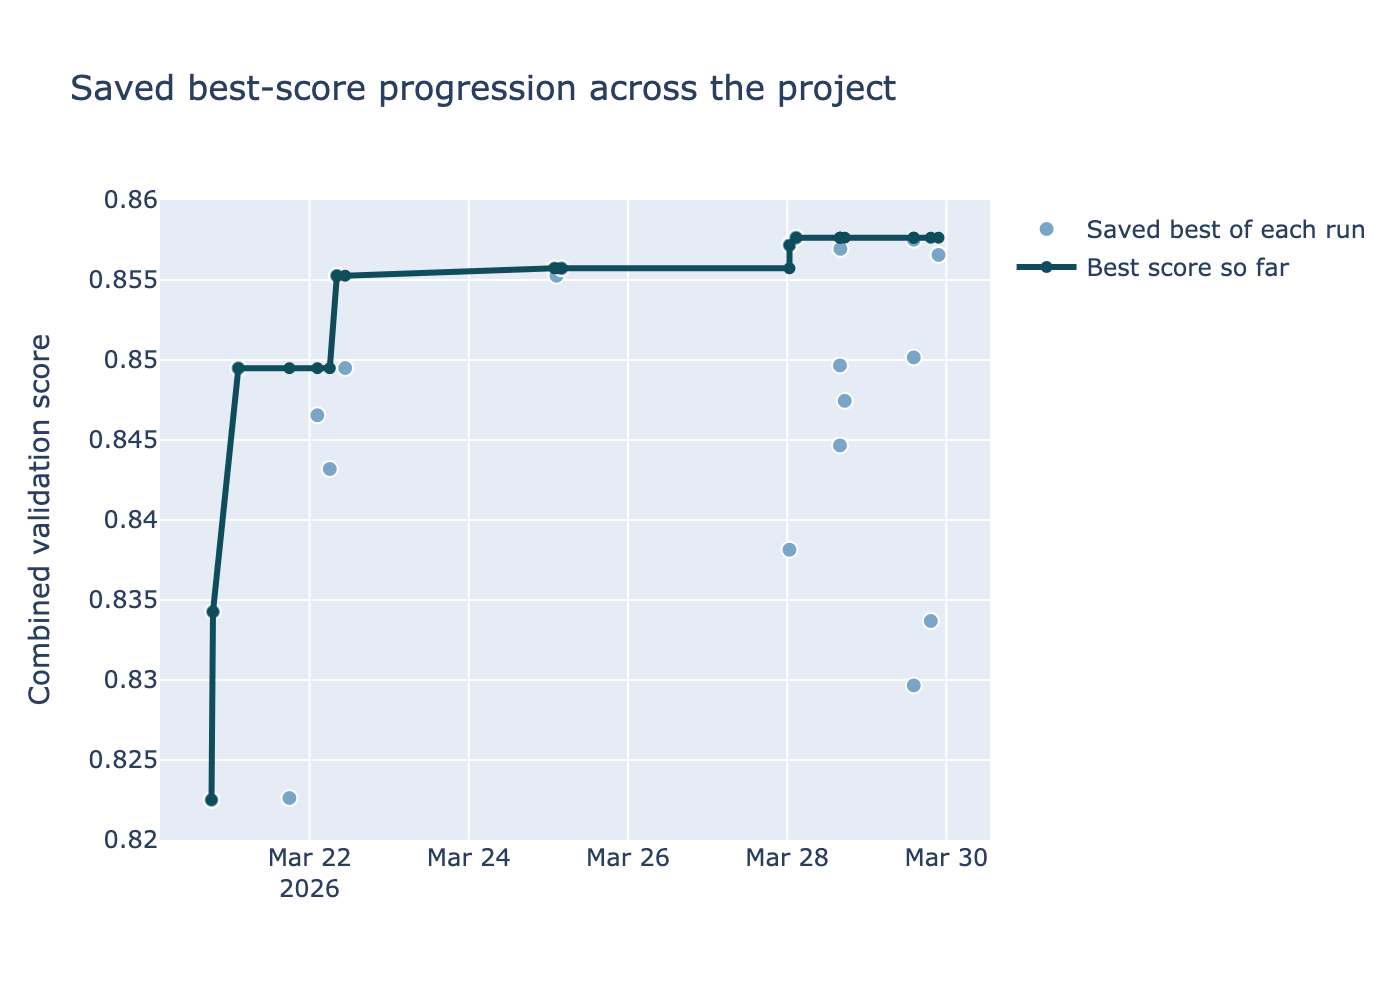
\includegraphics[width=\linewidth]{figures/methods_score_progression.png}
    \caption{Saved best-score progression across the project. The general pattern was steady upward motion, but the gains became smaller and more expensive late in the project.}
\end{figure}

\begin{figure}[H]
    \centering
    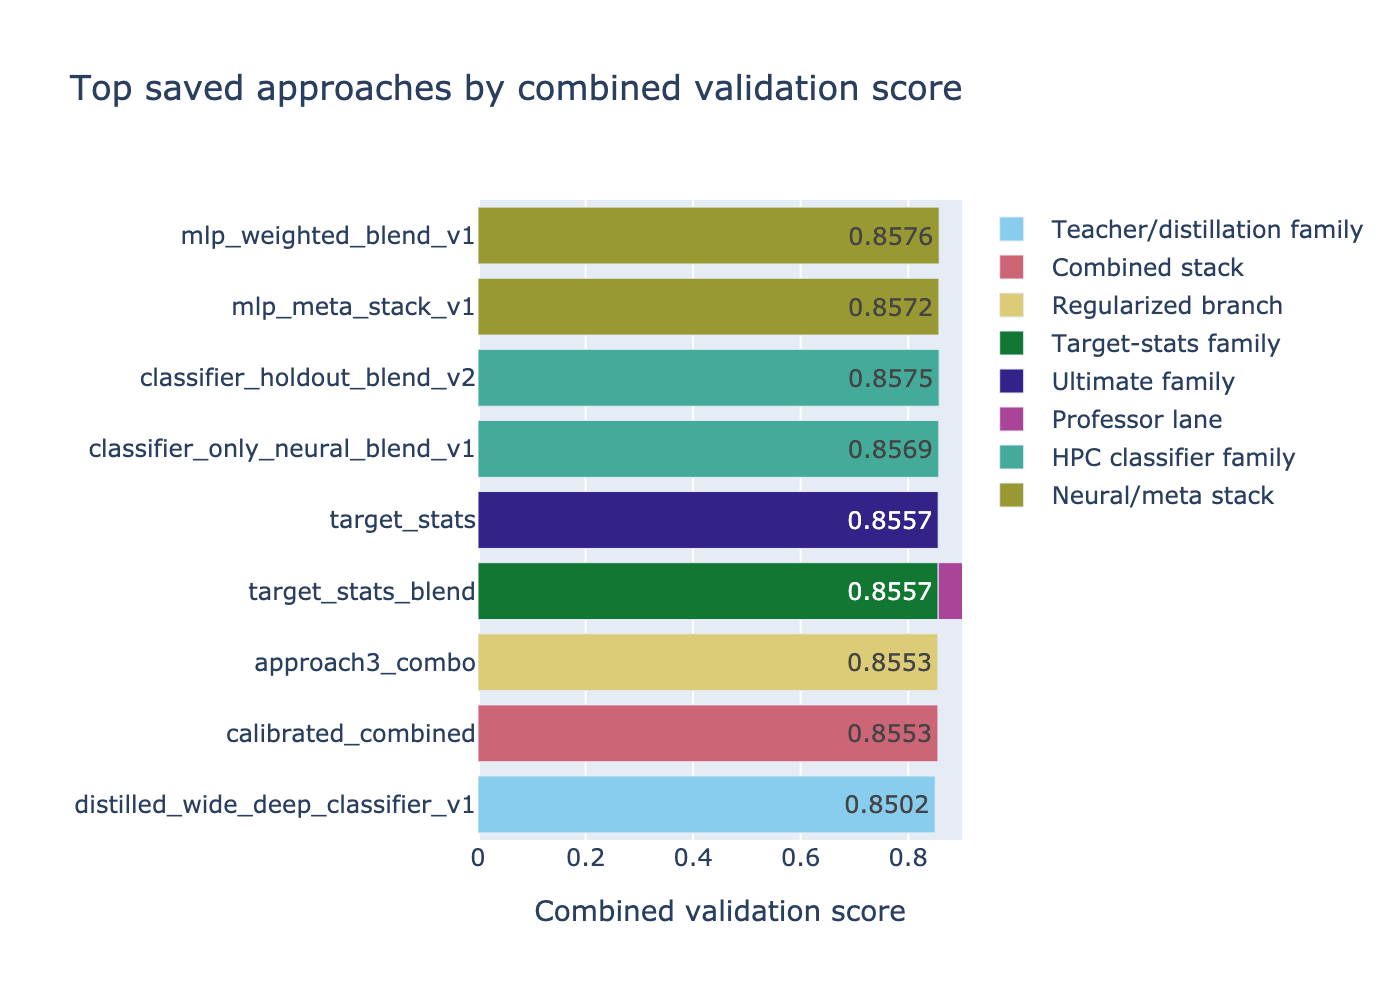
\includegraphics[width=\linewidth]{figures/methods_top_approaches.png}
    \caption{Top saved approaches by the combined validation metric. The strongest rows are not isolated single models; they are blends sitting on top of strong tabular sources.}
\end{figure}

Three takeaways kept repeating:

\begin{itemize}
    \item Stronger feature artifacts mattered more than cosmetic model swapping.
    \item The best local scores came from combinations of good branches, not from one heroic standalone model.
    \item The project improved when it stayed selective. The most expensive feature or model idea was not automatically the best one.
\end{itemize}

This is why the project eventually settled on a layered story: build a reliable tabular source first, then add a lighter combination layer on top if it earns its keep.

\section*{3. Compute, Runtime, And Public Calibration}

The project used both the MacBook and the MBZUAI HPC lab, but not for the same kind of work. Short MPS-supported experiments and compact meta models were comfortable on the Mac. Wider classifier families, cross-validated neural runs, and the professor lane made more sense on HPC, where the logs explicitly show workstations such as \texttt{ws-l5-031} and \texttt{ws-l5-032}.

\begin{figure}[H]
    \centering
    \begin{subfigure}[t]{0.58\linewidth}
        \centering
        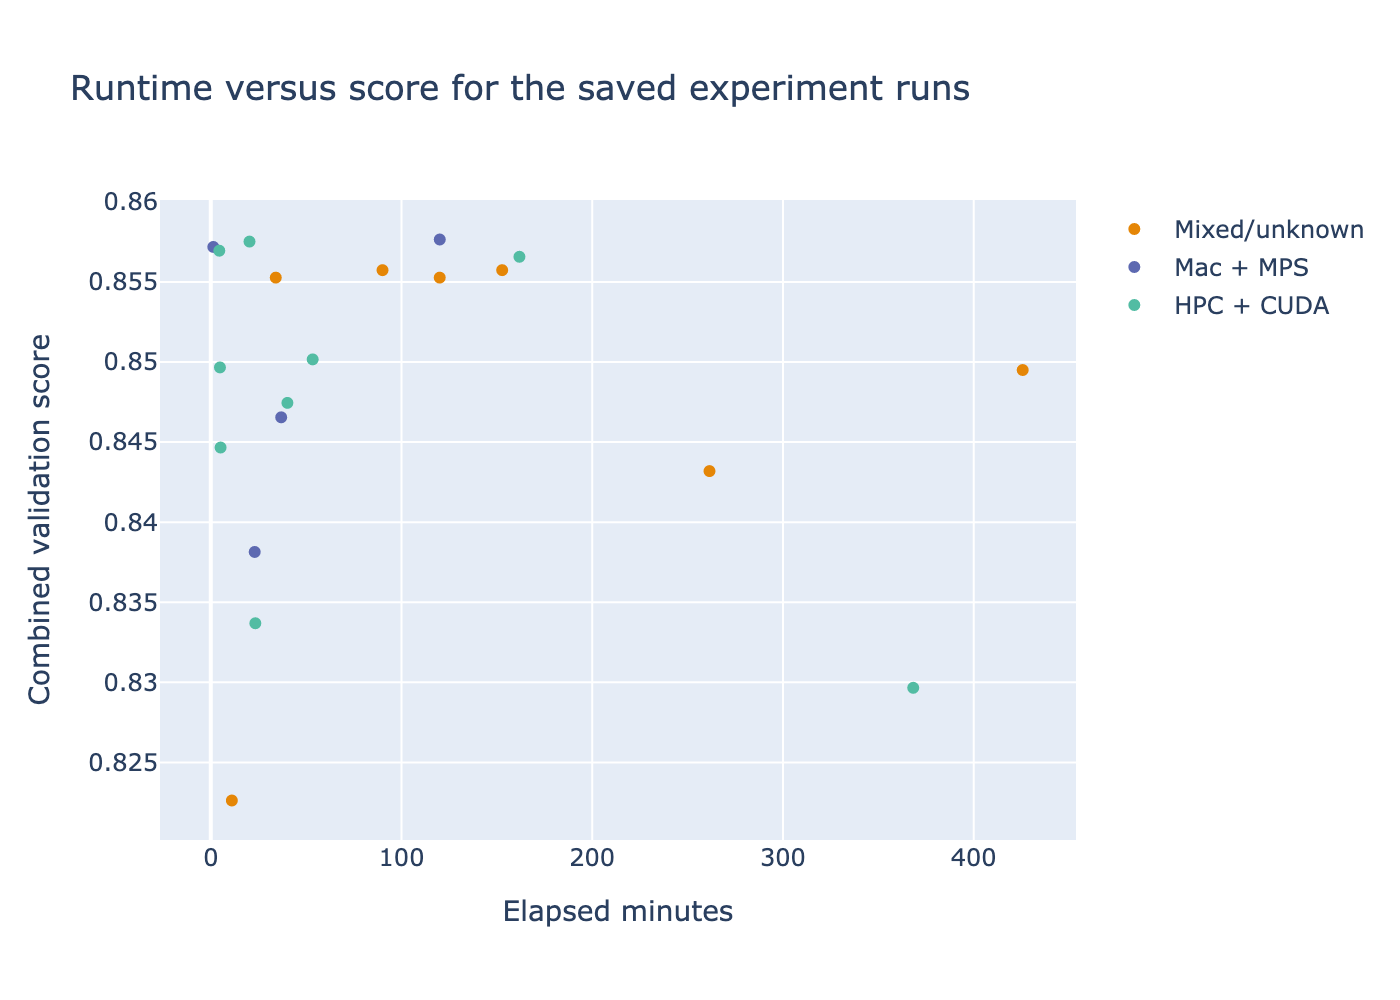
\includegraphics[width=\linewidth]{figures/methods_runtime_tradeoff.png}
        \caption{Runtime versus score for the saved runs.}
    \end{subfigure}\hfill
    \begin{subfigure}[t]{0.38\linewidth}
        \centering
        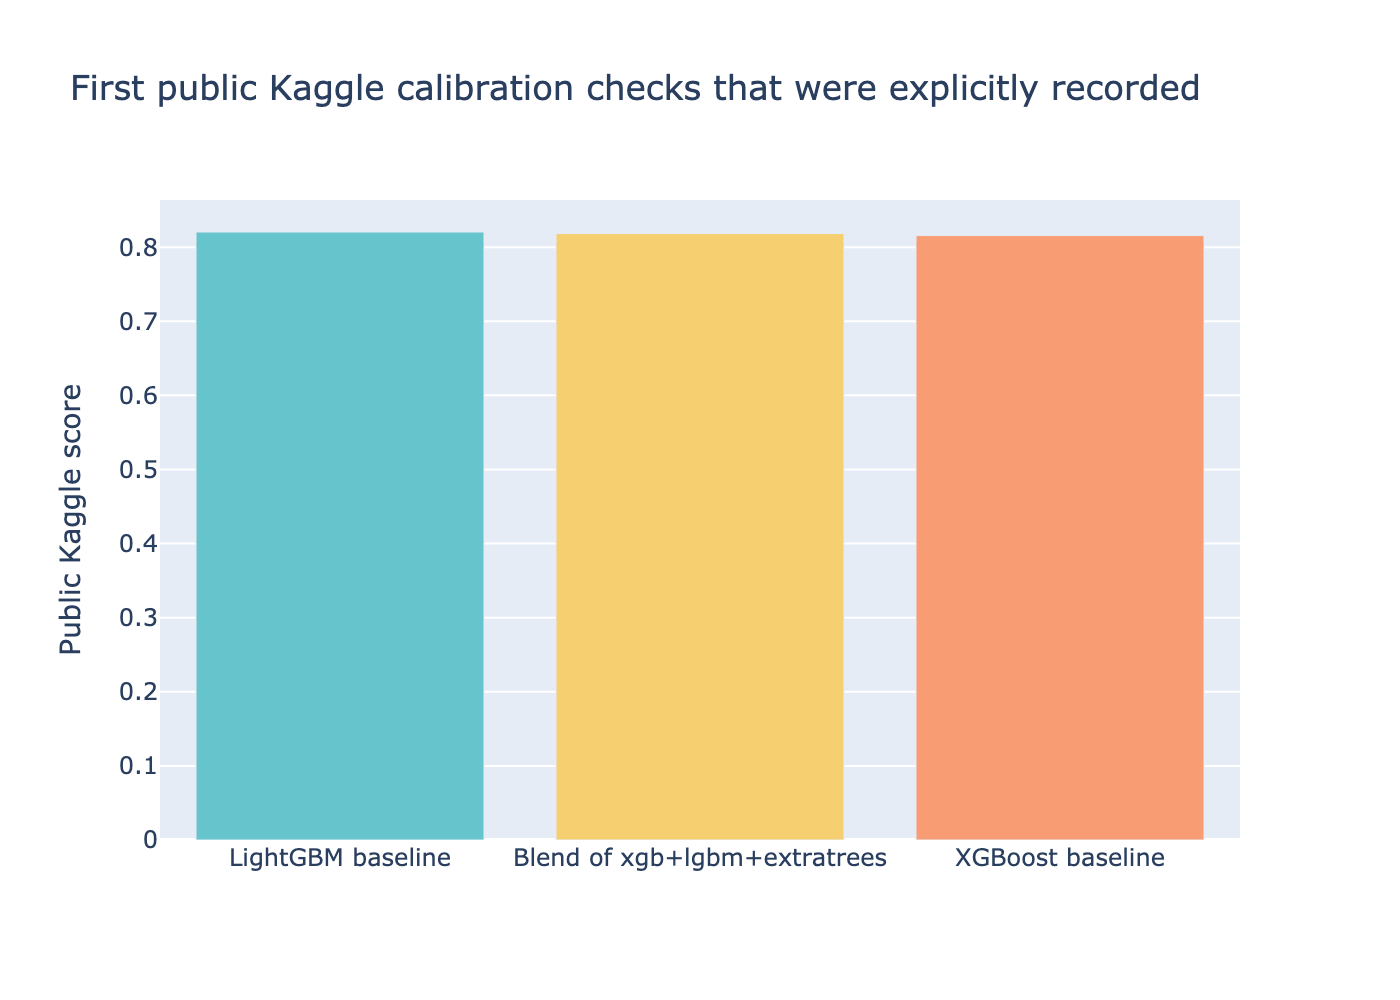
\includegraphics[width=\linewidth]{figures/methods_public_checks.png}
        \caption{The early public Kaggle checks that were explicitly recorded.}
    \end{subfigure}
    \caption{The project needed both local speed and cluster muscle. Public Kaggle checks were used sparingly, mostly to calibrate the local metric rather than replace it.}
\end{figure}

\rowcolors{2}{coolbg}{white}
\begin{table}[H]
    \centering
    \small
    \begin{tabularx}{\linewidth}{>{\bfseries}p{0.30\linewidth} >{\centering\arraybackslash}p{0.18\linewidth} >{\centering\arraybackslash}p{0.16\linewidth} X}
        \rowcolor{ink!12}
        Run & Score & Minutes & Compute note \\
        \texttt{mlp\_meta\_stack\_v1} & 0.857181 & 1.33 & Tiny Mac-side meta model; very cheap and surprisingly effective. \\
        \texttt{mlp\_weighted\_blend\_v1} & 0.857645 & 120.06 & Mac/MPS blend search; best local result that survived in the saved artifacts. \\
        \texttt{classifier\_holdout\_blend\_v2} & 0.857517 & 20.31 & HPC/CUDA run; strong late-stage competitor, especially on the classification side. \\
        \texttt{approach\_professor\_target\_stats} & 0.856566 & 161.83 & HPC refresh of the target-stats branch after the professor suggestions. \\
        \texttt{tree\_teacher\_classifier\_bagging\_v2} & 0.829660 & 368.29 & Expensive and technically interesting, but not a practical winner on the project metric. \\
    \end{tabularx}
    \caption{A few runtime snapshots show the real trade-off: some of the best ideas were cheap, while some of the most expensive ones were mainly educational.}
\end{table}

The public leaderboard was helpful, but only in small doses. The first Kaggle calibration on March 20 showed that the local ranking was useful: LightGBM was best publicly among the first three, the blend was close behind, and XGBoost trailed slightly. That was enough to justify keeping Kaggle as a checkpoint rather than turning the whole project into a submission lottery.

Later public scores were not kept with the same level of detail in the retained artifacts, so the second half of the project had to lean mostly on saved validation tables and training logs.

\section*{4. What Survived, What Stayed As Exploration}

\noindent
\begin{minipage}[t]{0.48\linewidth}
\softpanel{tealaccent}{%
\textbf{What clearly survived}
\begin{itemize}
    \item strong tabular feature artifacts, especially the target-stats substrate
    \item careful branch combination instead of single-model heroics
    \item lighter neural or meta layers used as finishers, not as total replacements
    \item splitting work sensibly across Mac/MPS and HPC/CUDA
    \item treating Kaggle submissions as calibration points rather than blind search
\end{itemize}}
\end{minipage}\hfill
\begin{minipage}[t]{0.48\linewidth}
\softpanel{ink}{%
\textbf{What mostly stayed as exploration}
\begin{itemize}
    \item fully replacing the strong tabular core with pure classifier-only neural ideas
    \item the most aggressive feature factories when they added more complexity than signal
    \item tree-teacher and distillation-style branches as final leaders
    \item the professor classical screen as a direct replacement for the best existing lanes
    \item any branch whose exact history was not preserved well enough to defend with artifacts
\end{itemize}}
\end{minipage}

\vspace{0.8em}

Overall, the project improved most when it emphasized disciplined iteration rather than isolated novelty. The strongest gains usually came from better feature artifacts, cleaner pruning, stronger tabular branches, and careful combination of those branches.

The professor-inspired lane still mattered. It widened the search space, improved the refreshed target-stats branch slightly, and forced the project to think more carefully about missingness and feature selection. But it behaved more like a good upstream research lane than like a full new winner.

For the final release, the overnight family was used as the main published pipeline rather than the absolute best local blend. Its performance remained strong, while its branch structure and artifact trail were substantially more stable than those of the later experimental hybrids.

\vspace{0.5em}

\softpanel{tealaccent}{%
\textbf{Final takeaways}
\begin{enumerate}
    \item The score story was mostly a story about better artifacts and better combinations, not about abandoning trees.
    \item The best local branch did exceed the released overnight lane, but the overnight family remained the more stable and reproducible final pipeline.
    \item Some old exact results are gone, but the overall trend is still clear from the saved score tables and logs.
    \item If the project were continued, the most sensible next step would be to keep the target-stats backbone, keep the professor lane as an upstream research branch, and only retune the final combiner when the upstream source truly improves.
\end{enumerate}}


\end{document}
